\section{Follow-ups}
\subsection{Monomial orderings}
\begin{frame}
    \textit{Are there any different monomial orderings in $K\left[x\right]$?}

    \begin{itemize}
        \item $\succ$ is a total order 
        \item $\alpha \succ \beta \Rightarrow \alpha + \gamma \succ \beta + \gamma$
        \item $\succ$ is a well-ordering
    \end{itemize}

    Obviously, either $1\succ 0$ or $0 \succ 1$; however, the latter is not a well-ordering.

    Why are we interested in well-ordering?

    \only<1>{\, }
    \only<2>{\textit{This property is used for proving termination of algorithms}}
\end{frame}

\begin{frame}
    $\alpha, \beta \in \mathbb{N}_0^n$, $W$ -- $k\times n, k\leq n$ matrix.
    
    Is $\alpha \succ \beta := W \alpha \succ_{lex} W\beta$ a monomial ordering?

    Ex:
    \[
        W = \begin{pmatrix} 1 & 1 &  \hdots & 1 & 1 \\ 1 & 0 & \hdots & 0  & 0 \\ 0 & 1 & \dots & 0  & 0 \\ \vdots & \vdots & \ddots &  \vdots & \vdots \\ 0 & 0 & \hdots & 1 & 0\end{pmatrix}
    \]
\end{frame}

\subsection{Quotient ring bases}
\begin{frame}
    $K\left[x_1,\dots,x_n\right], I=\left\langle f_1, \dots, f_k\right\rangle, \dim I = 0 \Rightarrow \dim \faktor{K\left[\dots\right]}{I} < \infty$


    $$B=\left\{x^\alpha: x^\alpha\not\in LT\left(I\right)\right\}$$
    
    How do we enumerate $B$?

    \begin{itemize}
        \item $\forall i\, K\left[x_i\right]\cap I \neq \varnothing$
        \item Only finite number of elements left
        \item Then -- use Gr\"obner bases' leading monomials
    \end{itemize}
   
    \pause
    $$I=\left\langle 2x^2+y^2+3y-12, x^2-y^2+x+3y-4\right\rangle$$
    \pause
    $$G_{lex}=\left\{9\mathbf{y^4}-18y^3-13y^2+30y-8, 2\mathbf{x}-3y^2+3y+4\right\}$$
    \pause
    $$G_{grevlex}=\left\{3\mathbf{y^2}-2x-3y-4, 3\mathbf{x^2}+x+6y-16\right\}$$
\end{frame}

\section{Theory}
\subsection{Matrix Buchberger's algorithm}
\begin{frame}
    $I=\left\langle f_1,\dots,f_k\right\rangle$, $f_j\in K\left[x_1,\dots,x_n\right]$, $\succ$

    $X = \left\{x^\alpha\right\}$

    Let us define $\mathcal{S}=\left\{x^\alpha f_i\right\}$ and write their coefficients as a ``matrix'' $S$

    $$S X = \mathbb{0}$$

    \begin{itemize}
        \item Transform $S$ to reduced row-echelon form $T$
        \item Let $C$ be a set of polynomials in $T$ whose leading term is not a multiple of leading term of other polynomial
        \item $\Rightarrow C$ is a Gr\"obner basis of $I$
    \end{itemize}
\end{frame}

\begin{frame}
    Infinite ``matrices'' sound so wrong\dots

    Known bounds:
    \begin{itemize}
            \item Reduced Gr\"obner basis degree (1990): $$2\left(\frac{d^2}{2}+d\right)^{2^{n-1}}$$
            \item Required power of $x^\alpha$ (2014): $$2\left(\frac{d^2}{2}+d\right)^{2^{n-1}}+\sum_{j=0}^{n-1}\left(k d\right)^{2j}$$
    \end{itemize}

    If we already know, how ``original'' Buchberger's algorithm ``works'' on this set of polynomials, we can significantly tighten these boundaries
\end{frame}

\subsection{Design of closed-form solvers}
\begin{frame}
    Reducing to row-echelon form is no better than polynomial divison (in $\mathbb{R}\left[x_1,\dots,x_n\right]$)

    Known facts:
    \begin{itemize}
        \item (provable) For each system of equations $f_1,\dots,f_k\in\mathbb{Q}\left[x_1,\dots,x_n\right]$ there exists $p$ s.t. Buchberger's algorithm works ``the same'' for the corresponding system in $\mathbb{Z}_p$
        \item Some classes of systems have similar order of polynomial reduction for wide range of coefficient values
        \item With $p\gg 3$ it is very unlikely to obtain ``unlucky'' set of coefficients
    \end{itemize}
\end{frame}

\begin{frame}
    Offline phase:
    \begin{enumerate}
        \item Re-formulate problem in $\mathbb{Z}_p$
        \item Compute Gr\"obner basis in $\mathbb{Z}_p$
        \item Record s-pairs, quotient ring basis, leading monomials, etc
    \end{enumerate}

    Online phase:
    \begin{enumerate}
        \item Create elimination template by ``shifting'' original polynomials
        \item Perform matrix-based reduction
        \item Extract multiplication operator matrix
        \item Extract solutions from eigenvalues/eigenvectors
    \end{enumerate}
\end{frame}

\subsection{Eigenvalues and eigenvectors (solution extraction)}
\begin{frame}
    $$K\left[x_1,\dots,x_n\right]; V\left(f_1,\dots,f_k\right); I=I(V); \dim I = 0; R=\faktor{K\left[\dots\right]}{I}$$

    With $f \in K\left[\dots\right]$ we can define a linear operator:
    $$T_f:R\rightarrow R$$
    $$p\mapsto f p$$

    Then, if $\lambda,p$ are corresponding eigenvalue and eigenvector
    $$T_f p = \lambda p \Rightarrow \left(f\left(\mathbf{x}\right)-\lambda\right)p\in I$$

    So, each $\lambda$ corresponds to $f\left(\mathbf{x}\right)$ (for some $\mathbf{x}\in V$)

    For example, let $f=x_j$; then eigenvalues correspond to $\mathfrak{x}_j$ for $\mathbf{x}=\left(\mathfrak{x}_1,\dots,\mathfrak{x}_n\right)^\top\in V$

    Obviously(?!), in monomial basis, eigenvectors of $T_f$ correspond (up to scale) to $\left(\mathbf{x}^\alpha\right)$
\end{frame}



\section{Practice}
\subsection{Tools}
\begin{frame}
    Tools:
    \begin{itemize}
        \item Offline phase:
            \begin{itemize}
                \item \href{http://www2.macaulay2.com/Macaulay2/}{Macaulay2}
                \item \textit{Your favourite} symbolic math system
            \end{itemize}
        \item Online phase: any library that supports QR \& Eigenvalue decompositions
    \end{itemize}
\end{frame}

\subsection{Relative pose}
\begin{frame}
    Relative pose problem:
    \only<1>{
    $$
    \begin{cases}
        R \in \mathcal{SO}3 \\
        t\in S^2 \\
        x_\ell^\top \left[t\right]_\times R x_r =  \alpha x_\ell^\top E x_r = 0\\
    \end{cases}
    $$
    which is equal to
    $$
    \begin{cases}
        \det\left(E\right)=0\\
        2EE^\top E -\tr\left(E\right)E'E=\mathbb{0} \\
        x_\ell^\top E x_r = 0\\
    \end{cases}
    $$}

    $x_\ell^\top E x_r = 0$ is linear in $E$; \pause let's extract $E$ as:
    $$E=x\cdot X + y\cdot Y + z\cdot Z + W$$
    where $X$, $Y$, $Z$, $W$ are basis-vectors for nullspace of corresponding linear operator
    $$
    \begin{cases}
        \det\left(E\right)=0\\
        2EE^\top E -\tr\left(E\right)E'E=\mathbb{0} \\
        E=x\cdot X + y\cdot Y + z\cdot Z + W
    \end{cases}
    $$
\end{frame}

\begin{frame}
    In Macaulay2:
    \only<1>{
    \lstinputlisting{sections/p5p.m2}
}
    \only<2>{
        \lstinputlisting{sections/p5p.out}
    }
\end{frame}

\begin{frame}
    $$
    \begin{cases}
        \det\left(E\right)=0\\
        2EE^\top E -\tr\left(E\right)E'E=\mathbb{0} \\
        E=x\cdot X + y\cdot Y + z\cdot Z + W
    \end{cases}
    $$

    In GRevLex: no additional polynomials required!

    Lead terms:  $\left\{z^3, yz^2, xz^2, y^2z, xyz, x^2z, y^3, xy^2, x^2y, x^3\right\}$

    Basis in quotient ring: $\left\{1, x, x^2, xy, xz, y, y^2, yz, z, z^2\right\}$
\end{frame}


\subsection{Quadric intersection}
\begin{frame}
    $$
    \begin{cases}
        f_1(x,y)=ax^2+bxy+cy^2+dx+ey+f =0 \\
        f_2(x,y)=gx^2+hxy+ky^2+lx+my+n = 0 \\
    \end{cases}
    $$

    \textit{How many solutions we would like to get?}\pause -- 4
    \pause
    Basis in quotient ring: $\left\{1,x,y,y^2\right\}$

    Lead terms: $\left\{xy, x^2, y^3\right\}$

    Macaulay2 reports, that degree-4 polynomials were required
\end{frame}

\begin{frame}
    Insights that we've got from examining problem in $\mathbb{Z}_p$ with  Macaulay2:
    \begin{itemize}
        \item Elimination template (non-minimal) can be constructed from polynomials $f_1$, $f_2$ multiplied by $\left\{1,x,y,x^2,xy,y^2\right\}$.
    
        \item Multiplication by $x$: $1\mapsto x$, other monomials are mapped outside the basis.
    \end{itemize}
\end{frame}

\begin{frame}
    \begin{figure}
        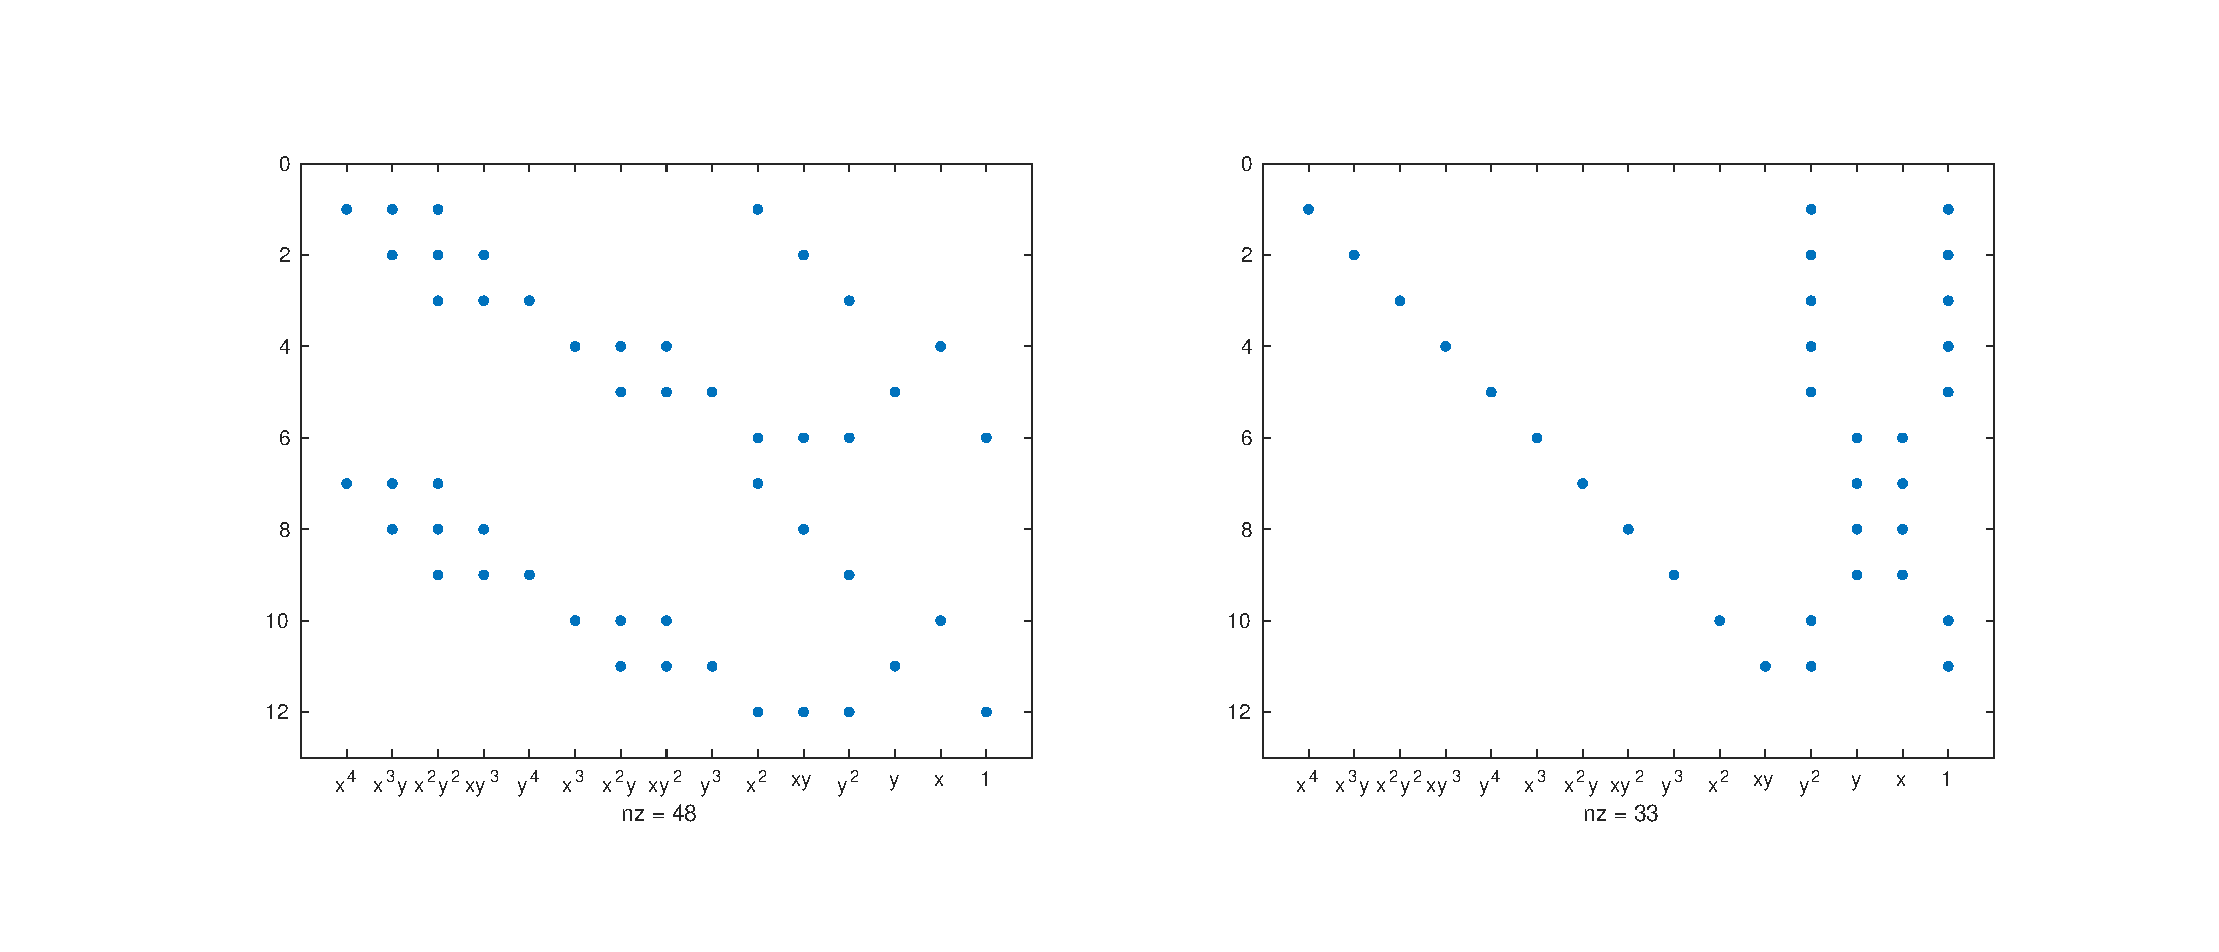
\includegraphics[width=1.\textwidth]{sections/quad_templates.eps}
        \caption{Macaulay-matrix based Buchberger's algorithm in action}
    \end{figure}
\end{frame}


\subsection{Tips \& tricks}
\begin{frame}
    \begin{itemize}
        \item Rotation parameterization
            \begin{itemize}
                \item Unit quaternions are double-cover
                \item 3-DoF non-unit quaternion parameterization
            \end{itemize}
        \item Constraint enforcement in  $\mathbb{Z}_p$
        \item Offline phase might be partially automated
    \end{itemize}
\end{frame}

